\section{Discovering the latent basis of DMs}
\label{sec:sec3}
In this section, we explain how to extract a latent structure of \exspace{} using differential geometry. 
First, we introduce a key concept in our method: the {\it pullback metric}. 
Next, by adopting the local Euclidean metric of \ehspace{} and utilizing the pullback metric, we discover the local latent basis of the \exspace{}. 
Moreover, although the direction we found is {\it local}, we show how it can be applied to other samples via parallel transport. 
Finally, we introduce $\vx$-space guidance for editing data in the \exspace{} {to enhance the quality of image generation.}

% Moreover, We also construct global latent basis using the {\it \frechet{} mean} of local semantic bases. 
% First, we use the {\it pullback metric} to characterize the geometrical structure of \exspace{}, adopting the local Euclidean metric of \ehspace{} to identify local semantic latent subspaces. 
% This is a way to give a space without a metric a spatial characterization using a space with a known metric. 
% Next, we adopt the local Euclidean metric of \ehspace{} to identify local semantic latent subspace for individual samples in \exspace{}. 
% Note that the \exspace{} is semantically sparse, but the subspace we found is semantically dense. 
% In Section 4, we show that the discovered direction within the semantic latent subspace can be exploited for editing. 
% Moreover, We also construct global latent basis using the {\it \frechet{} mean} of local semantic bases. 
% Finally, we introduce $\mathbf{x}$-space guidance for editing with better quality.
% Third, we found the homogenity across local semantic subspace discovered at various samples. From this observation, we construct global semantic directions by deriving the \frechet{} mean of the local semantic directions of individual samples. 
% We use the global semantic directions to manipulate any sample to have the same interpretable features.
% Finally, we introduce a technique called $x$-space guidance to edit sample with better quality.

%%% ICML ver
% This section explains how we extract the interpretable directions in the latent space of DMs using differential geometry. 
% First, we adopt the local Euclidean metric of \ehspace{} to identify semantic directions for individual samples in \exspace{}.
% Second, we find global semantic directions by averaging the local semantic directions of individual samples. Then, we use the global directions to manipulate any sample to have the same interpretable features.
% Finally, we introduce a normalization technique to prevent distortion.

% \begin{figure}[!t]
%     \centering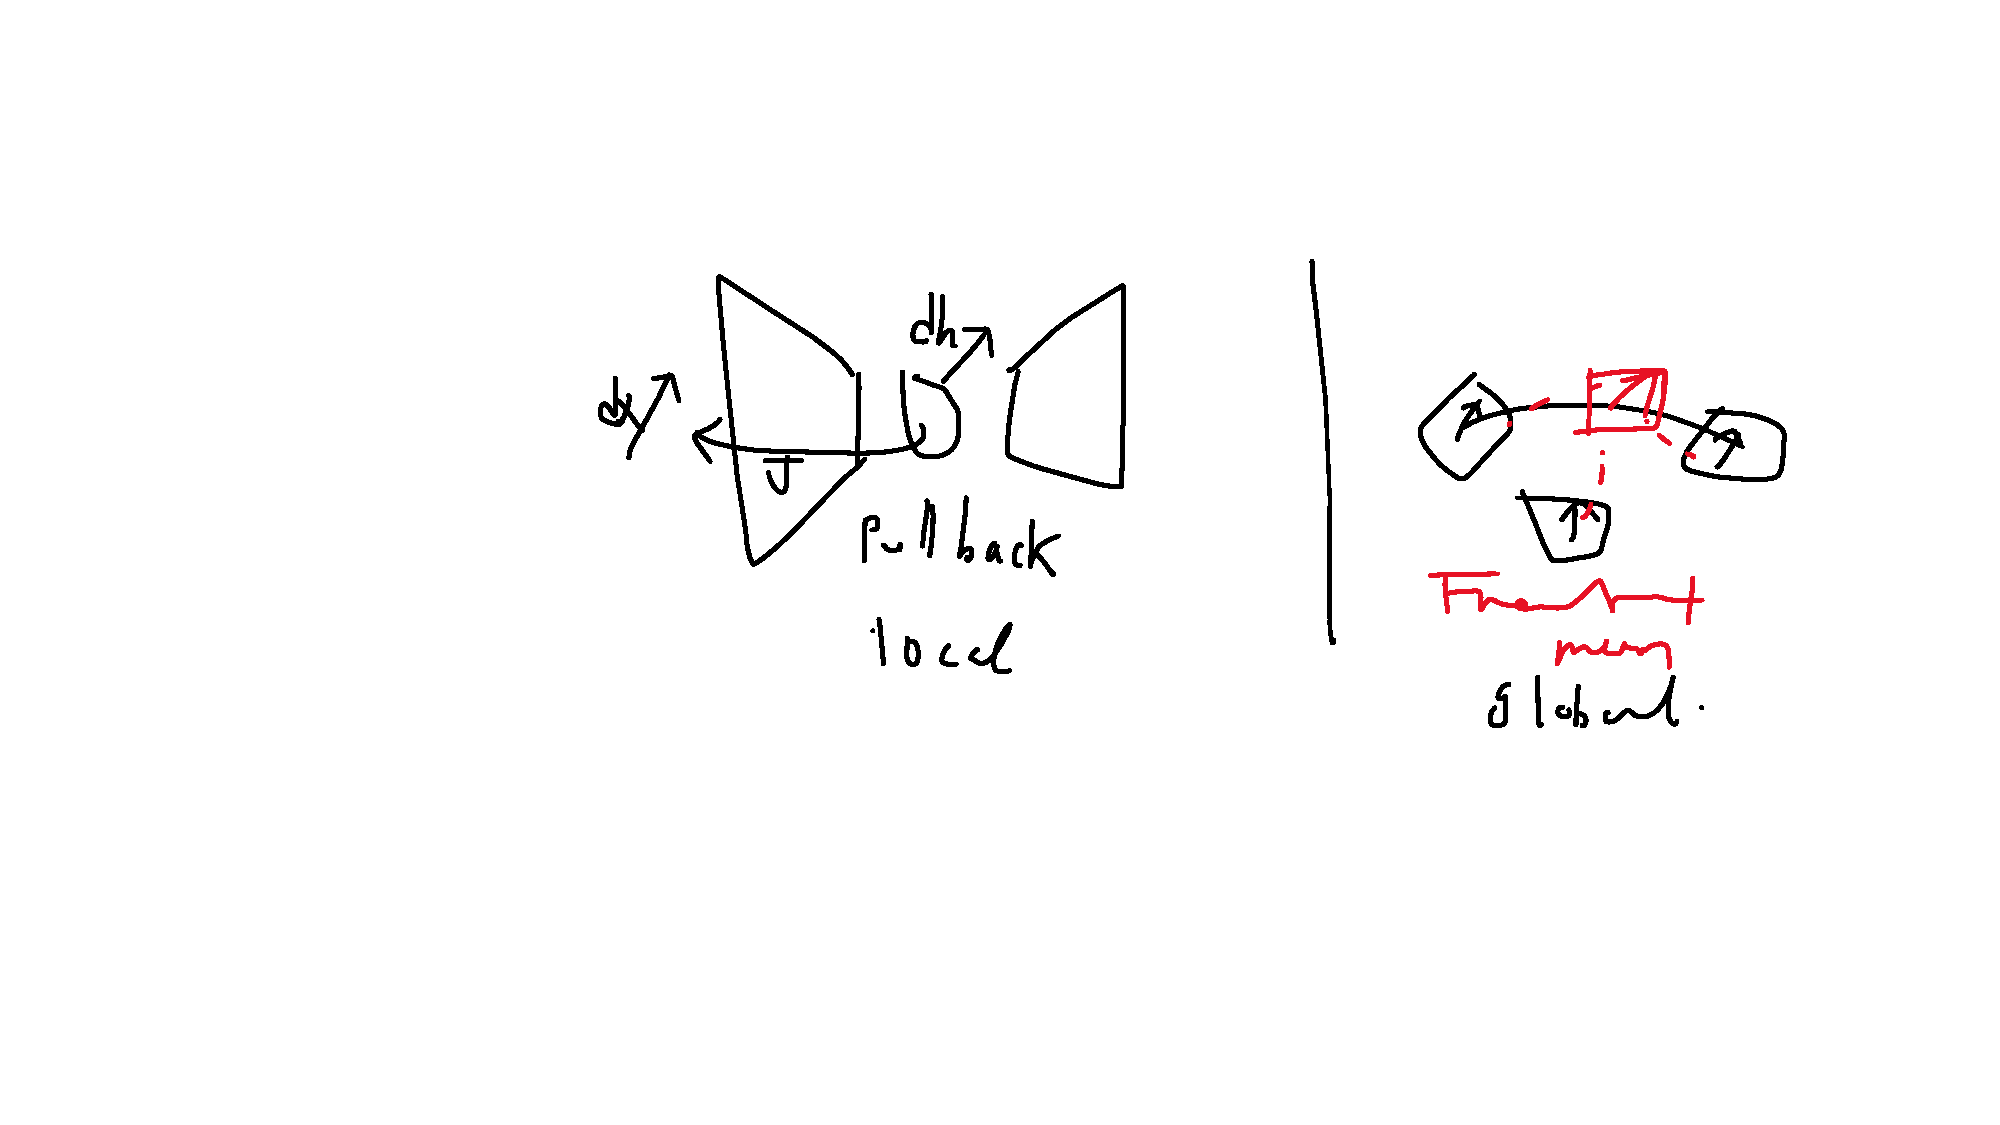
\includegraphics[width=0.8\linewidth]{figure/method_explain.pdf}
%     \caption{
%     \textbf{Conceptual illustration of our editing procedure.} 
%     It consists of two parts: (\textcircled{1} $\sim$ \textcircled{4}) discovering semantic latent directions using pullback metric and (\textcircled{5} $\sim$ \textcircled{8}) editing samples multiple times through geodesic shooting.
%     \textcircled{1} Map a sample in $\mathcal{X}$ into a tangent space $\mathcal{T}_\mathbf{h}$ in $\mathcal{H}$. 
%     \textcircled{2} Choose a direction in $\mathcal{T}_\mathbf{h}$.
%     \textcircled{3} Find its corresponding direction in $\mathcal{X}$ using $\jacx{}^{-1}$.
%     \textcircled{4} Edit the sample by adding the discovered direction after normalizing to a predefined length.
%     \textcircled{5} Map the edited sample to a new tangent space $\mathcal{T}_{\mathbf{h}'}$ in $\mathcal{H}$ for multiple editing.
%     \textcircled{6} Using parallel transport, move the direction chosen in \textcircled{2} to the new tangent space $\mathcal{T}_{\mathbf{h}'}$.
%     \textcircled{7}-\textcircled{8} Repeat \textcircled{3}-\textcircled{4}. And then repeat \textcircled{5}-\textcircled{8}.
% }
%     \vspace{-1em}
%     \label{fig:method_figure}
% \end{figure}

% \begin{figure}[!t]
%     \centering
%     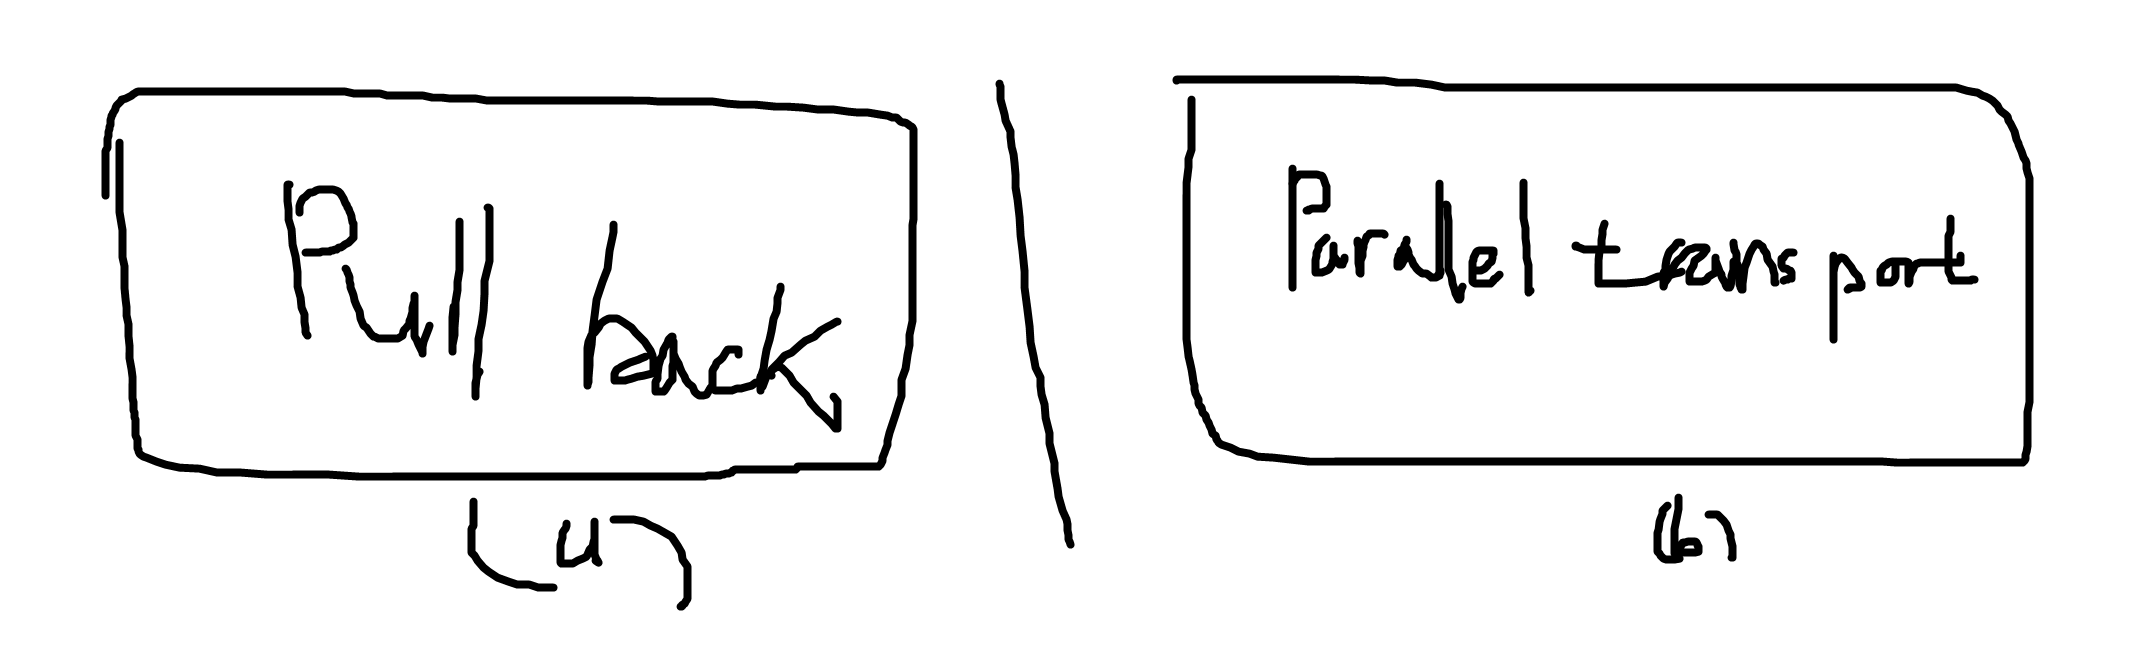
\includegraphics[width=1\linewidth]{figure/tmp_concept.png}
%     \caption{\textbf{Local (uncond + SD)} 
%     We find semantic directions in the latent space $\vx_t$ in an unsupervised fashion relying on Riemannian geometry between $\vx_t$ and $\vh_t$. $\mathcal{H}$ denotes the bottleneck layer and $f$ indicates the frozen encoder of a U-Net. 
%     The found directions manipulate the semantics of the resulting images.
%     }
%     \vspace{-1em}
%     \label{fig:local_basis_text}
% \end{figure}

\subsection{Pullback metric} \label{sec:pullback}
% In this subsection, we explain how to extract a local latent basis of \exspace{}, and their corresponding local tangent basis of \ehspace{} using differential geometry. 
% First, we introduce a key concept in our method: the pullback metric. 
% The pullback metric is a mathematical tool to define a metric on a space by exploiting the metric structure of another metric space.
% Next, we adopt the local Euclidean metric of \ehspace{} to identify local semantic latent subspace for individual samples in \exspace{}. 

We consider a curved manifold, \exspace{}, where our latent variables $\mathbf{x}_t$ exist. 
The differential geometry represents $\mathcal{X}$ through patches of tangent spaces, $\tanxspace{}$, which are vector spaces defined at each point $\mathbf{x}$. 
Then, all the geometrical properties of $\mathcal{X}$ can be obtained from the inner product of $||d\mathbf{x}||^2 = \langle d{\mathbf{x}},d{\mathbf{x}} \rangle_\mathbf{x}$ in $\tanxspace{}$.
However, we do not have any knowledge of $\langle d{\mathbf{x}},d{\mathbf{x}} \rangle_\mathbf{x}$.
It is definitely not a Euclidean metric. Furthermore, samples of $\mathbf{x}_t$ at intermediate timesteps of DMs include inevitable noise, which prevents finding semantic directions in $\tanxspace{}$.

Fortunately, \citet{kwon2022diffusion} observed that \ehspace{}, defined by the bottleneck layer of the U-Net, exhibits local linear structure.
% Fortunately, \citet{kwon2022diffusion} observed that \ehspace{}, defined by the bottleneck layer of the U-Net, exhibits \yh{semantically} local linearity.
% Henceforth, we denote \ehspace{} as $\mathcal{H}$.
This allows us to adopt the Euclidean metric on $\mathcal{H}$.
In differential geometry, when a metric is not available on a space, {\it pullback metric} is used.
If a smooth map exists between the original metric-unavailable domain and a metric-available codomain, the pullback metric is used to measure the distances in the domain space.
Our idea is to use the pullback Euclidean metric on $\mathcal{H}$ to define the distances between the samples in $\mathcal{X}$.

DMs are trained to infer the noise $\mathbf{\epsilon}_t$ from a latent variable $\mathbf{x}_t$ at each diffusion timestep $t$. 
Each $\mathbf{x}_t$ has a different internal representation $\mathbf{h}_t$, the bottleneck representation of the U-Net, at different $t$'s.
The differentiable map between $\mathcal{X}$ and $\mathcal{H}$ is denoted as $f : \mathcal{X} \rightarrow \mathcal{H}$.
Hereafter, we refer to $\mathbf{x}_t$ as $\mathbf{x}$ for brevity unless it causes confusion. It is important to note that our method can be applied at any timestep in the denoising process.
%$f$ gives a linear map $\nabla_{\mathbf{x}} \mathbf{h} : \tanxspace{} \rightarrow \tanhspace{}$ between the domain and codomain tangent spaces.
{We consider a linear map, $\tanxspace{} \rightarrow \tanhspace{}$, between the domain and codomain tangent spaces.}
%The differential geometry then defines a linear map between the tangent space $\tanxspace{}$ at $\mathbf{x}$ and corresponding tangent space $\tanhspace{}$ at $\mathbf{h}$. The 
This linear map can be described by the {\it Jacobian} $J_{\mathbf{x}} = \nabla_{\mathbf{x}} \mathbf{h}$
which determines how a vector $\mathbf{v} \in \tanxspace{}$ is mapped into a vector $\mathbf{u} \in \tanhspace{}$ by
$\mathbf{u} = J_{\mathbf{x}} \mathbf{v}$. 
% In practice, the Jacobian can be computed from automatic differentiation of the U-Net.
% However, since the Jacobian of too many parameters is not tractable, we use a sum-pooled feature map of the bottleneck representation as our $\mathcal{H}$. 

Using the local linearity of $\mathcal{H}$, we assume the metric, $||d\mathbf{h}||^2 = \langle d\mathbf{h}, d\mathbf{h} \rangle_\mathbf{h} = d\mathbf{h}^{\tran} d\mathbf{h}$ as a usual dot product defined in the Euclidean space.
To assign a geometric structure to $\mathcal{X}$, we use the pullback metric of the corresponding $\mathcal{H}$.
In other words, the norm of $\mathbf{v} \in \tanxspace{}$ is measured by the norm of corresponding codomain tangent vector:
\begin{equation} \label{eq:pullback}
\begin{aligned}
||\dx{}||^2_\text{pb} \triangleq  \langle \dh{}, \dh{} \rangle_{\mathbf{h}} = \dx{}^{\tran} \jacx{}^{\tran} \jacx{}\dx{}.
\end{aligned}
\end{equation}

% \subsection{\yh{Find the local semantic latent directions}}
% \subsection{\yh{Extracting the semantic directions and editing}}
% \subsection{Extraction of semant directions}

% \yh{This subsection describes how we extract semantic latent directions using the pullback metric, and how we construct semantic latent subspace using discovered directions. The overall process is illustrated in \fref{fig:method_figure}.}

%%% ICML ver
% \label{sec:method_local}
% This subsection describes how we extract semantic latent directions using the pullback metric, and how we edit samples for multiple times given the meaningful directions by geodesic shooting. The overall process is illustrated in \fref{fig:method_figure}.


\begin{figure}[!t]
    \centering
    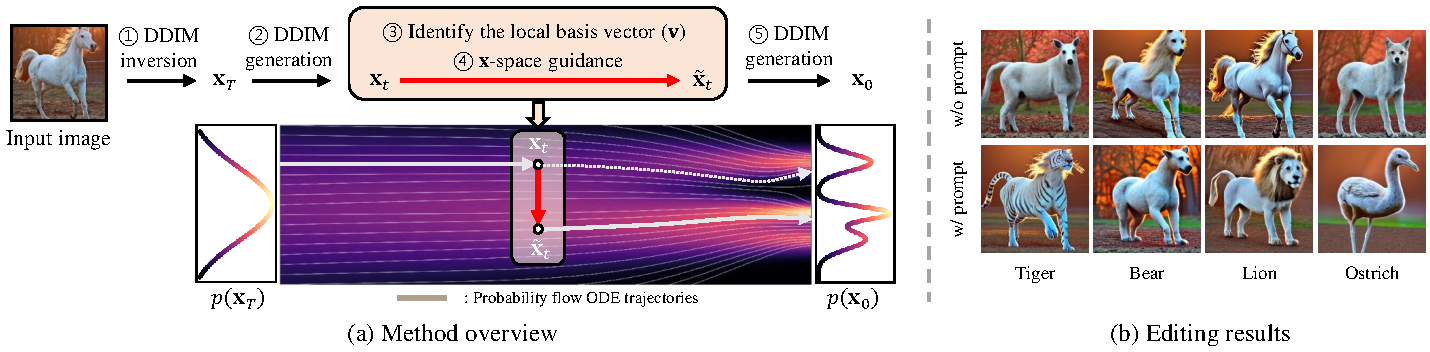
\includegraphics[width=1\linewidth]{figure/method_rebuttal_circle.pdf}
    % 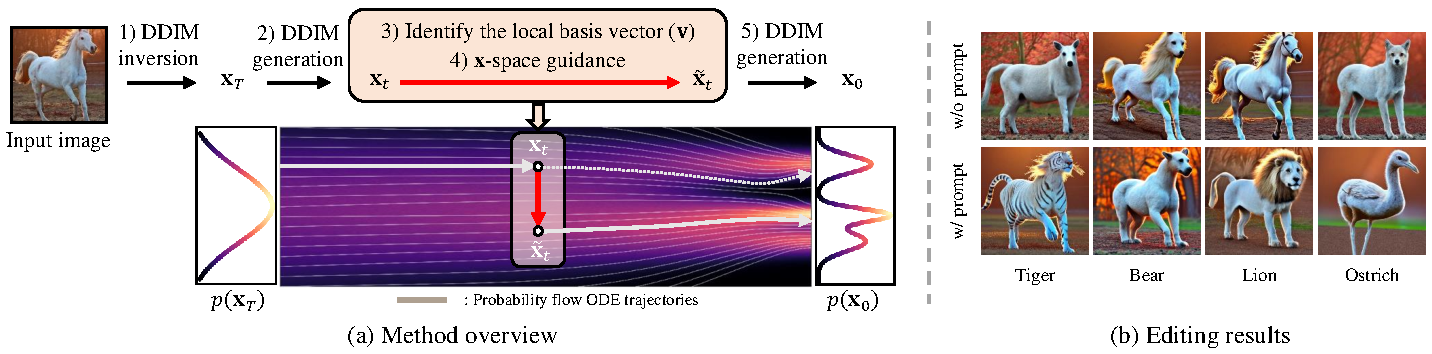
\includegraphics[width=1\linewidth]{figure/method_rebuttal_2.pdf}
    \vspace{-1em}
    \caption{\textbf{Image editing with the discovered latent basis.} 
    (a) Schematic depiction of our image editing procedure. 
    \modify{①} An input image is subjected to DDIM inversion, resulting in an initial noisy sample $\mathbf{x}_T$. 
    \modify{②} The sample $\mathbf{x}_T$ is progressively denoised until reaching the point $t$ through DDIM generation. 
    \modify{③} Subsequently, the local latent basis $\{\mathbf{v}_1, \cdots, \mathbf{v}_n\}$ is identified by using the pullback metric. 
    \modify{④} This enables the manipulation of the sample $\mathbf{x}_t$ along one of the basis vectors using $\mathbf{x}$-space guidance. 
    \modify{⑤} The DDIM generation concludes with the progression from the modified latent variable $\tilde{\mathbf{x}}_t$.
    (b) Examples of edited images using a selected basis vector. The latent basis vector \modify{could be} conditioned on prompts \modify{and it} facilitates text-aligned manipulations.
    }
    \vspace{-1em}
    \label{fig:method}
\end{figure}


\subsection{Finding local latent basis}
Using the pullback metric, 
{
we define the local latent vector $\mathbf{v} \in \tanxspace{}$ {that shows a large variability in $\tanhspace{}$}.
We find a unit vector $\mathbf{v}_1$ that maximizes $||\dx{}||^2_\text{pb}$.
}
% It can be interpreted as the first eigenvector of $\jacx{}^{\tran} \jacx{} = V \Lambda^2 V^{\top}$.
By maximizing $||\dx{}||^2_\text{pb}$ while remaining orthogonal to $\mathbf{v}_1$, one can obtain the second unit vector $\mathbf{v}_2$. This process can be repeated to have $n$ latent directions of $\{\mathbf{v}_1, \mathbf{v}_2, \cdots, \mathbf{v}_n \}$ in $\mathcal{T}_{\mathbf{x}}$. 
In practice, $\mathbf{v}_i$ corresponds to the $i$-th right singular vector from the singular value decomposition {(SVD)} of $\jacx{} = U \Lambda V^{\tran}$, i.e., $J_{\vx} \vv_{i} = \Lambda_{i} \vu_{i}$. 
Since the Jacobian of too many parameters is not tractable, we use a \textit{power method} \cite{golub2013matrix,miyato2018spectral,haas2023discovering} to approximate the SVD of $\jacx{}$
{(See \aref{appendix:comparisons} for the time complexity and \aref{appendixsec:algorithm} for the detailed algorithm).} 

{Henceforth, we refer to $\mathcal{T}_{\mathbf{x}}$ as a local latent subspace, and $\{\mathbf{v}_1, \mathbf{v}_2, \cdots, \mathbf{v}_n \}$ as the corresponding local latent basis.}
\begin{align}
    \mathcal{T}_{\mathbf{x}} \triangleq \text{span} \{\mathbf{v}_1, \mathbf{v}_2\, \cdots, \mathbf{v}_n\},~\text{where}~\mathbf{v}_i~\text{is}~i\text{-th right singular vector of}~J_{\mathbf{x}}.
\end{align}

%%% ICML ver : construct Th in h space 
Using the linear transformation between $\tanxspace{}$ and $\tanhspace{}$ via the Jacobian $\jacx{}$, one can also obtain corresponding directions in $\mathcal{T}_{\mathbf{h}}$.
% \begin{align}
%     \vu{}_i = \frac{1}{\lambda_i} \jacx{} \mathbf{v}_i.
% \end{align}
% Here, we normalize $\vu{}_i$ by dividing the $i$-th singular value $\lambda_i$ of \jo{the diagonal matrix} $\Lambda$ to preserve the Euclidean norm $||\mathbf{u}_i||=1$. 
In practice, $\mathbf{u}_i$ corresponds to the $i$-th left singular vector from the {SVD} of $\jacx{}$.
After selecting the top $n$ (e.g., $n = 50$) directions of large eigenvalues, we can approximate any vector in $\mathcal{T}_{\mathbf{h}}$ with {a} finite basis, $\{\mathbf{u}_1, \mathbf{u}_2, \cdots, \mathbf{u}_n \}$.
When we refer to a local tangent space henceforth, it means the $n$-dimensional low-rank approximation of the original tangent space.
\begin{align} \label{eq:local_tangent_space}
    \mathcal{T}_{\vh} \triangleq \text{span} \{\vu_1, \vu_2\, \cdots, \vu_n\},~\text{where}~\vu_i~\text{is the}~i\text{-th left singular vector of }~J_{\vx}.
\end{align}

%% mingi ver
% \paragraph{\yh{Interpretation of local latent basis}}
%The set of local latent basis vectors, $\{\vv_1, \vv_2, \cdots, \vv_n\}$, obtained through our proposed method, can be seen as a `{\it signal}' that the model is particularly sensitive given $\vx$.
%% These vectors represent the directions in which the model's representation $\mathbf{h}$ undergoes the most significant changes, revealing the information that the model focuses on from $\mathbf{x}_t$ for a specific sample.
%On the other hand, the basis of local tangent space, represented as $\{\vu_1, \vu_2\, \cdots, \vu_n\}$, can be thought of as the corresponding `{\it representation}' linked to the signal.
{The collection of local latent basis vectors, $\{\vv_1, \vv_2, \cdots, \vv_n\}$, obtained through our proposed method, can be interpreted as a {\it signal} that the model is highly response to for a given $\vx$.
On the other hand, the basis of the local tangent space, denoted as $\{\vu_1, \vu_2\, \cdots, \vu_n\}$, can be viewed as the corresponding {\it representation} associated with the signal.
}

{In Stable Diffusion, the prompt also influences the Jacobian, which means that the local basis also depends on it. }
% We can utilize any prompt to obtain a local latent basis.
{
We can utilize any prompt to obtain a local latent basis, and different prompts create distinct geometrical structures.
}
% \mingi{In a conditional model, the local tangent space undergoes prompt-dependent modifications, allowing us to derive a specific basis by using the prompt as a condition of the model. Note that we can utilize any prompt to obtain a local latent basis.}
{For the sake of brevity, we will omit the word {\it local} unless it leads to confusion.}

% %%% YH ver start
% \yh{
% % The local latent basis $\{\vv_1, \vv_2\, \cdots, \vv_n\}$ discovered in our method can be considered to the signal to which the model is sensitive, given $\mathbf{x}_t$. 
% The set of local latent basis vectors $\{\vv_1, \vv_2, \cdots, \vv_n\}$ obtained through our approach can be  understood as a {\it signal} that the model is responsive to, given $\vx_t$. 
% % This interpretation underscores the relevance of these vectors in shaping the model's response to the input.
% % The local latent basis vectors $\{\vv_1, \vv_2, \cdots, \vv_n\}$ discovered by our method represent the signal to which the model responds when given input $\mathbf{x}_t$. This highlights the crucial role of these vectors in shaping the model's output.
% This subspace consists of the directions that result in the most significant change in the model's representation $\mathbf{h}$, revealing the information that the model is most attentive to from $\mathbf{x}_t$ for a given sample. 
% In this regard, the basis of local tangent space $\{\vu_1, \vu_2\, \cdots, \vu_n\}$ can be understood as the {\it representation} corresponding to the signal.
% }
% %%% YH ver end

%%% ICML ver
% So far, we extracted meaningful directions for editing $\mathbf{x}_t$ and construct local semantic subspace.
% However, these directions are {\it local}, and thus are only applicable to individual samples of $\mathbf{x}_t$.
% Thus, we need to obtain {\it global} semantic directions that have the same semantic meaning for every sample.
% Fortunately, we observed a large overlap between the latent directions of individual samples.
% This observation motivates us to hypothesize that \ehspace{} has global semantic directions.

% \paragraph{Iterative editing with geodesic shooting} 
% Now, we edit a sample with the $i$-th semantic direction through $\mathbf{x} \to \mathbf{x}' = \mathbf{x} + \gamma \mathbf{v}_i$, where $\gamma$ is a hyper-parameter 
% that controls the size of the editing.
% If we want to increase the editing strength, we need to repeat the same operation. However, this would not work because $\mathbf{v}_i$ may escape from the tangent space $\mathcal{T}_{\mathbf{x}'}$.
% Thus, it is necessary to relocate the extracted direction to a new tangent space.
% To achieve this, we use {\it parallel transport} that projects $\mathbf{v}_i$ onto the new tangent space $\mathcal{T}_{\mathbf{x}'}$. 
% Parallel transport moves a vector without changing its direction as much as possible, while keeping the vector tangent on the manifold~\cite{shao2018riemannian}.
% It is notable that the projection significantly modifies the original vector $\mathbf{v}_i$, because $\mathcal{X}$ is a curved manifold.
% However, $\mathcal{H}$ is relatively flat. Therefore, it is beneficial to apply the parallel transport in $\mathcal{H}$.

% To project $\mathbf{v}_i$ onto the new tangent space $\mathcal{T}_{\mathbf{x}'}$, we use parallel transport in $\mathcal{H}$. First, we convert the semantic direction $\mathbf{v}_i$ in $\mathcal{T}_{\mathbf{x}}$ to the corresponding direction of $\mathbf{u}_i$ in $\mathcal{T}_{\mathbf{h}}$. Second, we apply the parallel transport $\mathbf{u}_i \in \mathcal{T}_{\mathbf{h}}$ to ${\mathbf{u}'}_{i} \in \mathcal{T}_{\mathbf{h}'}$, where $\mathbf{h}' = f(\mathbf{x}')$. 
% The parallel transport has two steps. The first step is to project $\mathbf{u}_i$ onto a new tangent space. This step keeps the vector tangent to the manifold. The second step is to normalize the length of the projected vector. This step preserves the size of the vector.
% Third, we obtain $\mathbf{v}'_{i}$ by transforming $\mathbf{u}'_{i}$ into $\mathcal{X}$.
% Using this parallel transport of $\mathbf{v}_i \to \mathbf{v}'_i$ via $\mathcal{H}$, we can realize the multiple feature editing of $\mathbf{x} \to \mathbf{x}' = \mathbf{x} + \gamma\mathbf{v}_i \to \mathbf{x}'' = \mathbf{x}' + \gamma \mathbf{v}'_i $.
% Based on the definition of Jacobian, this editing process can be viewed as a movement in \ehspace{} with the corresponding direction, i.e., $\mathbf{h} \to \mathbf{h}' = \mathbf{h} + \delta \mathbf{u}_i \to \mathbf{h}'' = \mathbf{h}' + \delta \mathbf{u}'_i$.  `
% This iterative editing procedure is called {\it geodesic shooting}, since it naturally forms a geodesic ~\cite{shao2018riemannian}.
% \fref{fig:method_figure} summarizes the above procedure. 
% See \aref{appendixsec:algorithm} for details.

% \begin{figure}[!t]
%     \centering
%     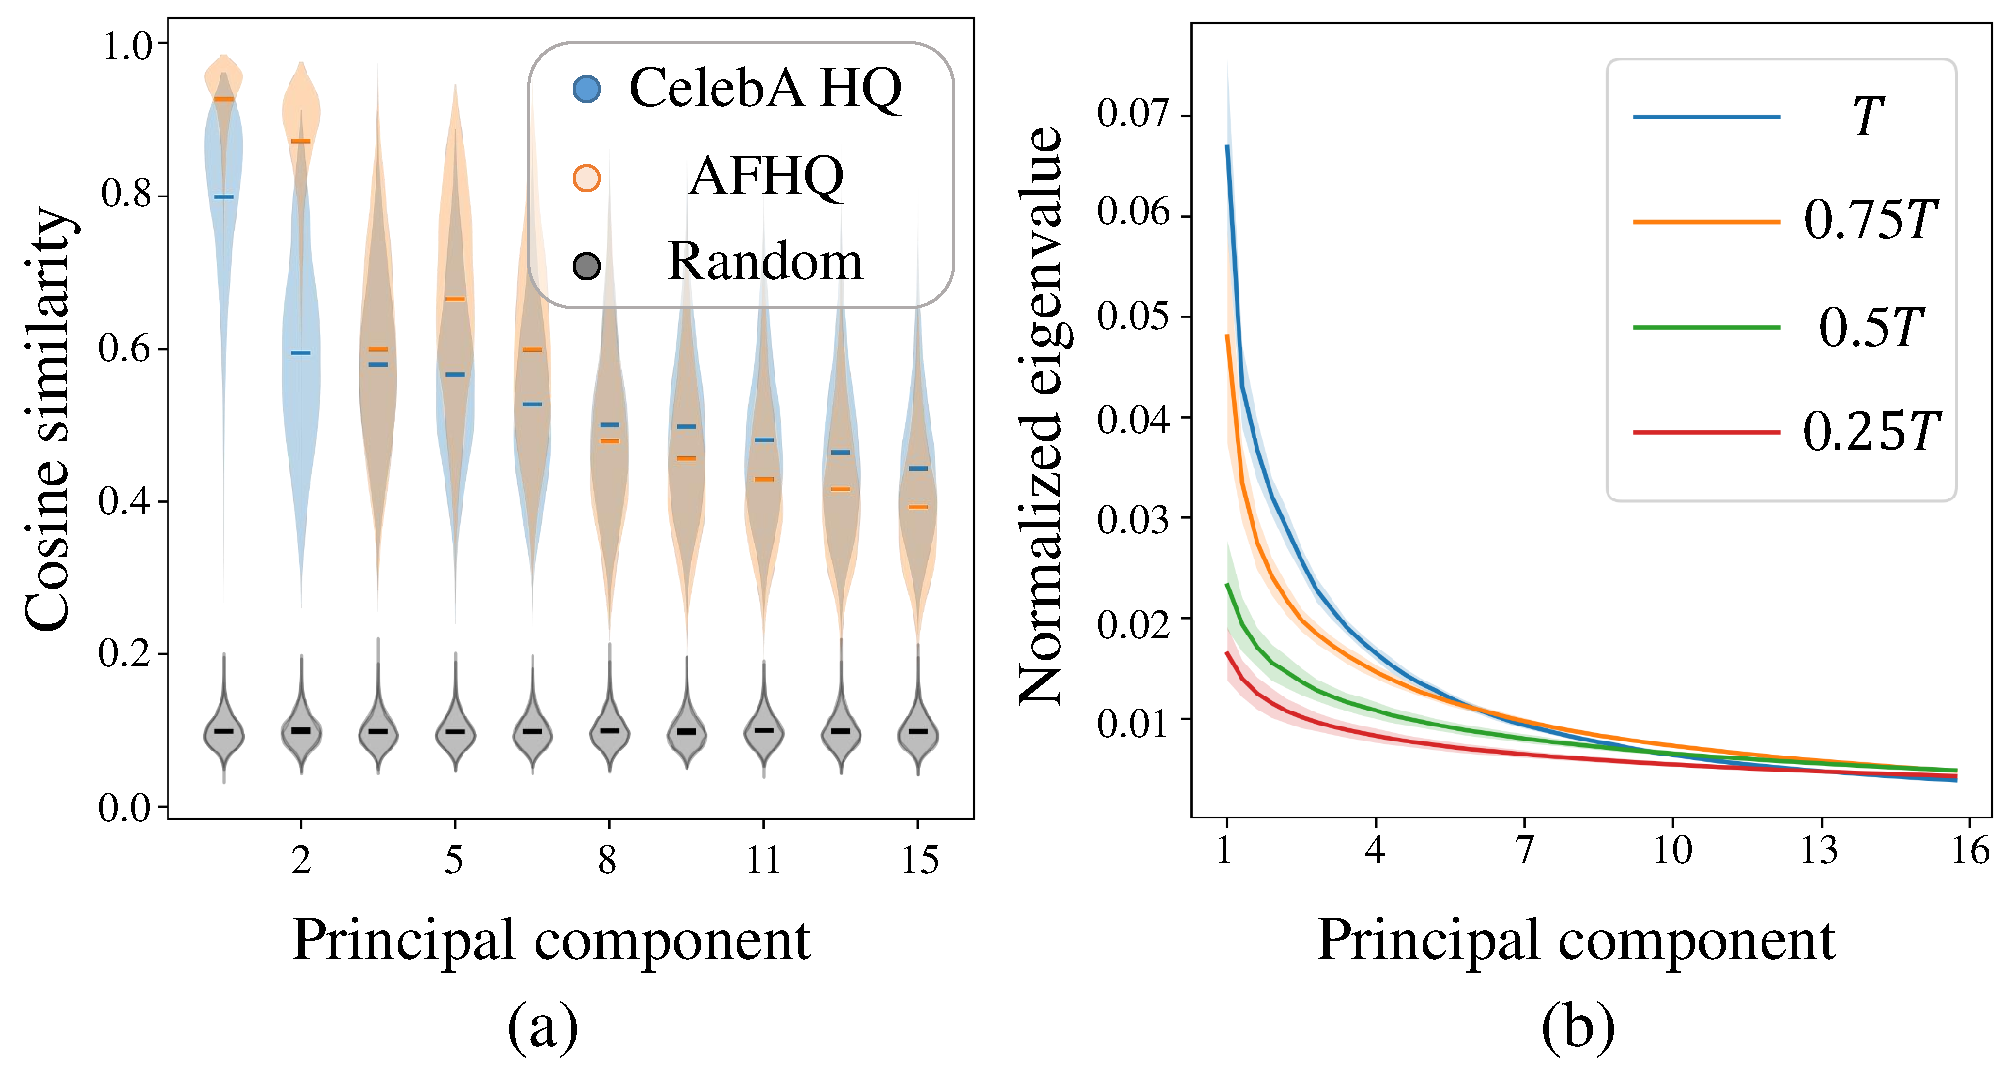
\includegraphics[width=1\linewidth]{figure/homogenity.pdf}
%     \caption{
%     \textbf{(a) Homogeneity across local directions from different images.} A distribution represents the statistics of maximum cosine similarities between the principal directions of pairs of 100 samples in $\mathbf{x}_T$.
%     The top principal directions better align than the rest.
%     The comparison with random directions (black) confirms that the similarity does not arise by chance.
%     \textbf{(b) Eigenvalue spectrum of $\jacx{}$ at different timesteps.}
%     Early timesteps ($t\approx T$) have larger top eigenvalues implying fewer but more eminent directions than later timesteps. 
%     }
%     \vspace{-1em}
%     \label{fig:homogenity}
% \end{figure}




\subsection{{Generating edited images with $\mathbf{x}$-space guidance}}
% \modify{찾은 basis를 어떻게 사용하는 건지에 대한 이야기임을 말하면서 글 다듬기.}
{A na\"ive approach for manipulating a latent variable $\mathbf{x}$ using a latent vector $\mathbf{v}$ is through simple addition, specifically $\mathbf{x}+\gamma\mathbf{v}$.
However, using the na\"ive approach sometime leads to noisy image generation.
% because the basis vectors are found in the space \exspace{} where the latent variables $\mathbf{x}$, that are prone to noise, exist.
To address this issue, instead of directly using the basis for manipulation, we use a basis vector that has passed through the decoder once for manipulation.
}
%To manipulate the latent variable $\mathbf{x}$ with a given local latent basis vector $\mathbf{v}$, the simple approach is adding basis to the latent variable, i.e. $\mathbf{x}+\gamma\mathbf{v}$. 
%However, \exspace{}, where we find the basis, is a noisy space by default and simple approach sometimes gives rise to noisy results. 
%To solve this problem, we use a basis vector for manipulation after going through the decoder once, instead of using the basis directly for manipulation.
The $\mathbf{x}$-space guidance is defined as follows
\begin{align}
\label{eq:xguidance}
    \tilde{\mathbf{x}}_{\text{XG}} = \mathbf{x} + \gamma[\epsilon_{\theta}(\mathbf{x}+\mathbf{v}) - \epsilon_{\theta}(\mathbf{x})]
\end{align}
where $\gamma$ is a hyper-parameter controlling the strength of editing and $\epsilon_{\theta}$ is a diffusion model. 
% \jo{(((g는 함수인가?)))}
Equation~\ref{eq:xguidance} is inspired by classifier-free guidance, but the key difference is that it is directly applied in the latent space \exspace{}.
{Our $\mathbf{x}$-space guidance provides qualitatively similar results to direct addition, 
\modify{while} it shows better fidelity. (See \aref{appendixsec:ablation_x_guidance} for ablation study.)}
% \yh{We provide an ablation study on this in \sref{}.}

\subsection{The overall process of image editing}
In this section, we summarize the entire editing process with five steps: 1) The input image is inverted into initial noise $\mathbf{x}_T$ using DDIM inversion. 2) $\mathbf{x}_T$ is gradually denoised until $t$ through DDIM generation. 3) Identify local latent basis $\{ \mathbf{v}_1, \cdots, \mathbf{v}_n \}$ using the pullback metric at $t$. 4) Manipulate $\mathbf{x}_t$ along the one of basis vectors using the $\mathbf{x}$-space guidance. 5) The DDIM generation is then completed with the modified latent variable $\tilde{\mathbf{x}}_t$. \fref{fig:method} illustrates the entire editing process. 

In the context of a text-to-image model, such as Stable Diffusion, it becomes possible to include textual conditions while deriving local basis vectors. 
% 이를 통해 DDIM inversion 이나 generation 때 text 에 의한 guidance 를 주지 않고도 text condition 에 맞는 editing 을 할 수 있게 된다.
\modify{
Although we do not use any text guidance during DDIM inversion and generation, a local basis with text conditions enables semantic editing that matches the given text.
% It enables semantic editing that matches the text conditions even without giving guidance based on text during DDIM inversion or generation.
}
% It aligns all the local basis vectors with the condition text. 
Comprehensive experiments can be found in Section 4.1.

% It is noteworthy that our approach \modify{needs no extra training}. Moreover, it achieves semantically meaningful image editing, only involving a traversal of the latent variable within a single timestep.
\modify{
It is noteworthy that our approach needs no extra training and simplifies image editing by only adjusting the latent variable within a single timestep.
}



\subsection{{Editing various samples with parallel transport}}

\modify{
Let us consider a scenario where our aim is to edit ten images, changing straight hair to curly hair. 
Due to the nature of the unsupervised image editing method, it is becomes imperative to manually check the semantic relevance of the latent basis vector in the edited results. 
% Considering the inherent characteristics of the unsupervised image editing method, it becomes imperative to manually inspect the semantic relevance of the latent basis vector within the edited results. 
Thus, to edit every samples, we have to manually find a straight-to-curly basis vector for individual samples.
% Therefore, for each editing task, we must manually identify a straight-to-curly basis vector specific to each image.
}

\modify{
One way to alleviate this tedious task is to apply the curly hair vector obtained from one image to other images. 
}
However, the basis vector $\vv \in \tanxspace{}$ obtained at $\vx$ cannot be used for the other sample $\vx'$ because $\vv \notin \mathcal{T}_{\vx'}$. 
% 왜냐면, 
% 이 번거로운 작업을 거쳐야 하는 이유는 우리가 local basis 를 찾았기 때문이다. 
% 우리가 a latent basis of $\tanxspace{}$ 에서 curly hair 방향을 찾더라도 
% So far, we extracted a latent basis of $\tanxspace{}$ and a tangent basis of $\tanhspace{}$ given {a} latent variable $\vx$. 
% Thus, 우리가 구한 direction 을 다른 sample 에 적용하기 위해선 it is necessary to relocate the extracted direction to a new tangent space.
% However, the basis vector obtained cannot be used for the other sample $\vx'$ because $\vv \notin \mathcal{T}_{\vx'}$. 
% If we do not use P.T., we have to manually find a straight-to-curly basis vector for individual samples. P.T. allows transporting a straight-to-curly basis vector in one sample to all other samples to edit all images with only one manual inspection.
Thus, in order to apply the direction we obtained to another sample, it is necessary to relocate the extracted direction to a new tangent space.
To achieve this, we use parallel transport that moves $\vv_i$ onto the new tangent space $\mathcal{T}_{\vx'}$.

Parallel transport moves {a tangent vector $\vu \in \tanhspace{}$ to $\vu' \in \mathcal{T}_{\vh'}$} without changing its direction as much as possible while keeping the vector tangent on the manifold \cite{shao2018riemannian}.
{It is notable that the parallel transport in curved manifold significantly modifies the original vector.
% It is notable that the projection significantly modifies the original vector $\mathbf{v}_i \in \tanxspace{}$, because $\mathcal{X}$ is a curved manifold.
Fortunately,} $\mathcal{H}$ is relatively flat. Therefore, it is beneficial to apply the parallel transport in $\mathcal{H}$.

We aims to move $\vv_i$ onto new tangent space $\mathcal{T}_{\mathbf{x}'}$, using parallel transport in $\mathcal{H}$.
First, we convert the latent direction $\vv_i \in \mathcal{T}_{\mathbf{x}}$ to the corresponding direction of $\vu_i \in \mathcal{T}_{\mathbf{h}}$.
Second, we apply the parallel transport $\vu_i \in \mathcal{T}_{\mathbf{h}}$ to ${\mathbf{u}'}_{i} \in \mathcal{T}_{\mathbf{h}'}$, where $\mathbf{h}' = f(\mathbf{x}')$. 
% Specifically, we consider the parallel transport along a geodesic between $\vh$ to $\vh'$.
In the general case, parallel transport involves iterative projection and normalization on the tangent space along the path connecting two points \cite{shao2018riemannian}.
However, in our case, we assume that \ehspace{} has Euclidean geometry. 
Therefore, we move $\vu$ directly onto $\mathcal{T}_{\mathbf{h}'}$ through projection, without the need for an iterative process.
Finally, transform $\mathbf{u}'_{i}$ into $\mathbf{v}'_i \in \mathcal{X}$.
% % Third, we obtain $\mathbf{v}'_{i}$ by transforming $\mathbf{u}'_{i}$ into $\mathcal{X}$.
Using this parallel transport of $\mathbf{v}_i \to \mathbf{v}'_i$ via $\mathcal{H}$, 
we can apply the local latent basis obtained from $\vx$ to edit or modify the input $\vx'$.


